% ------------ Two slopes method --------------------
\section{Two slopes method}
For a description of the two slopes method see \cite{Oliver}. \\ 
This method is shown unless the software was compiled without Fortran support.  \\

\begin{figure}[ht]
  \centering
  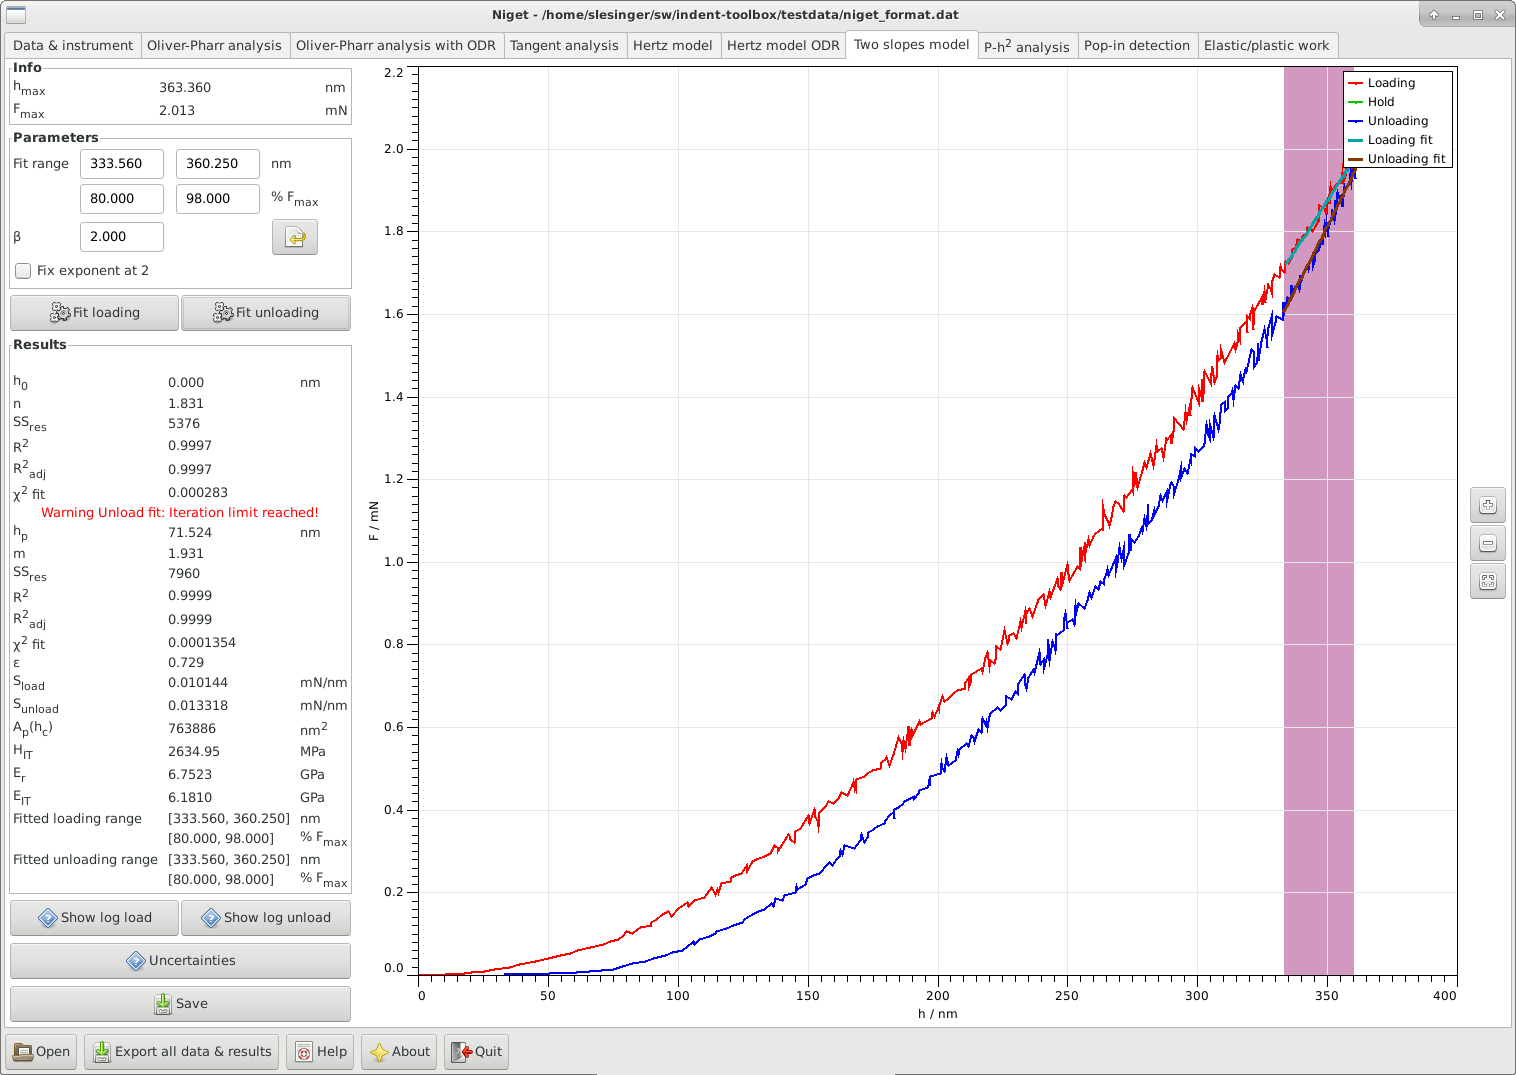
\includegraphics[width=\textwidth]{images/screen-twoslopes}
  \caption{Two slopes analysis using orthogonal data regression}
\end{figure}

\subsection{Window}
The window consists of several blocks:
\begin{itemize}
 \item \emph{Info} displays the maximum depth and force during the indentation
 \item \emph{Parameters} shows the selected range in nm and in \% of the maximum force, and the correction $\beta$. 
        \begin{itemize}
          \item[-] The fitting range can be selected either using the mouse or typing in the range entries. The range can be defined either in nm or in percent of the maximum force. 
                   It is often recommended to use the range 80--98 \% F$_\mathrm{max}$ for the fit, see section \ref{slopes_calc}.  
          \item[-] The parameter $\beta$ accounts for any deviations from the axisymmetric case and is used in the calculation of the reduced modulus in equation \eqref{eq:Er}. 
                   Currently, the default value is no correction $\beta = 1.0$. The value supplied by the user is saved in the settings and can be reset to its default value.
          \item[-] Check box, whether or not the exponent of the loading curve should be fitted or fixed at the theoretical value 2, see \ref{slopes_calc}.
          \end{itemize}
 \item \emph{Fit} buttons for indepedent fitting of the loading and unloading curves, see section \ref{slopes_calc} for details of the calculation.
 \item \emph{Results} displays all results in the following order: 
       the auxiliary depth parameter $h_0$, the power $n$ of the power law loading function, 
       the residual depth $\hp$, the power $m$ of the power law unloading function, the parameter $\varepsilon$, 
       the loading slope $\Sload$, the unloadingslope $\Sunload$, 
       the contact area $\Ap(\hc)$, the indentation hardness $H_{IT}$, the contact modulus $E_r$, the indentation modulus $E_{IT}$ and the ranges used for the fitting procedures.
       The variables are described in detail in section \ref{slopes_calc}. Warnings are displayed if the fittings procedures failed.
 \item \emph{Uncertainties} show the uncertainty analysis window, see section \ref{slopes_unc}.
 \item \emph{Show log load} Show the report about the fitting procedure of the loading curve in a separate window.  The reports are saved to files \emph{fit.log.slopes.load.err} and \emph{fit.log.slopes.load.rpt}. 
 \item \emph{Show log unload} Show the report about the fitting procedure of the unloading curve in a separate window.  The reports are saved to files \emph{fit.log.slopes.unload.err} and \\ \emph{fit.log.slopes.unload.rpt}. 
 \item \emph{Save} save parameters and results to given file. 
 \item \emph{Graph} display the unloading curve and the fitted curves. Stepwise zooming/unzooming can be performed by selecting a range with the mouse and pressing the \emph{Zoom}/ \emph{Unzoom} buttons. The graph is restored to its original size by the \emph{Restore} button.
\end{itemize}

\subsection{Procedure} \label{slopes_calc}
The two slopes method combines the standard Oliver Pharr method and the quadratic loading curve to avoid the need of the contact area.
\begin{enumerate} 
 \item 
 Fit the upper part of the loading curve with a power law function
$$
F = \gamma (h - h_0)^n.
$$
using orthogonal least squares as implemented in the package ODRPACK95 \cite{odrpack95}. The range should be approx. 85--98 \% F$_\mathrm{max}$. The exponent $n$ can be kept fixed at its theoretical value 2.
 \item 
 Fit the upper part of the unloading curve with a power law function
$$
F = \alpha (h - \hp)^m.
$$
using orthogonal least squares as implemented in the package ODRPACK95 \cite{odrpack95}. The range should be approx. 85--98 \% F$_\mathrm{max}$. All three parameters are fitted.
\item The auxiliary parameter $\varepsilon$ is calculated from the power $m$ as in \eqref{eq:eps}
\item The slopes at the maximum depth are calculated as
\begin{eqnarray} \label{eq:Stwo}
\Sload &=& n \frac{ \Fmax}{\hmax-h_0} \\
\Sunload &=& m \frac{ \Fmax}{\hmax-\hp} 
\end{eqnarray}
\item 
The contact area, indentation hardness and contact modulus are calculated as
\begin{eqnarray}
 \Ap(\hc) &=& C_0 \Fmax^2 \left( \frac{2 \Sunload -\beta \varepsilon \Sload}{\Sunload \Sload} \right)^2 \\
 \Hit &=& \frac1{C_0 \Fmax} \left( \frac{\Sunload \Sload}{2 \Sunload -\beta \varepsilon \Sload} \right)^2 \\
 \Er &=& \frac1{2 \beta \Fmax}  \sqrt{\frac \pi{C_0}} \frac{\Sunload^2 \Sload}{2 \Sunload -\beta \varepsilon \Sload}
\end{eqnarray}
with $C_0$ the coefficient of the $h^2$ term in the area calibration function and $\beta$ a geometric correction term. Currently, we use $\beta = 1$.
\item
The indentation modulus can be calculated from \eqref{eq:Eit}

\end{enumerate}

